% !TeX root = ./jvk-blatt1.tex

% l.47 Play-Button


\excercise{Programmstart}

\begin{Infobox}[Infoboxen]
	Infoboxen sind dazu da, dir abseits der Aufgabenstellung immer wieder nützliche Informationen zu den Aufgaben auf den Weg zu geben. Hier relevante Dinge erklärt, meistens auch unter dem Einsatz von Beispielen.\\
	Damit sie, verglichen zu der eher schlichten Dokumentenstruktur von \LaTeX, etwas hervorstechen, sind sie in einem \color{javaInstances} schönen Farbton eingeklammert.
\end{Infobox}

\begin{Infobox}[How-To: Projekt Import in Eclipse]
    \begin{enumerate}[label=\arabic*.]
		\item Entpacke die heruntergeladene \texttt{\jvkpackage} Datei in einem geeigneten Ordner.\\
		$\rightarrow$ \textbf{Windows:} Machen einen Rechtsklick auf die Datei und wähle dann
		\fbox{Alle extrahieren...}$\to$\fbox{Extrahieren}
		aus.\\
        $\rightarrow$ \textbf{Linux:} Öffne die Shell deines Vertrauens, navigiere in den Downloads Ordner und führe dann
		\texttt{\textdollar~unzip \jvkpackage}
		aus\\
        $\rightarrow$ \textbf{Apple:} Öffne die Zip-Datei im Finder und entpacke sie durch einen einfachen Doppelklick.
        \item Starte nun Eclipse. Um das Projekt zu importieren, klicke zuerst auf \fbox{File} $\to$ \fbox{Import...}.
        \item Wähle in der Ordner-Auswahl \fbox{Maven}$\to$\fbox{Existing Maven Projects}. Klicke dann auf \fbox{Next >}.
        \item Drücke oben rechts auf \fbox{Browse...} und navigiere in das Verzeichnis, in welchem Du die \jvkpackage-Datei entpackt wurde.
        \item Stelle sicher, dass der Projektname im \textit{Projects} Bereich des Fensters auftaucht.
        \item Wähle zu guter Letzt noch \fbox{Finish} aus.
        \item Nachdem sich das Import-Fenster geschlossen hat, solltest du das Projekt nun im \textit{Package Explorer} auf der links an der Seite des Eclipse-Fensters sehen.
        \item Damit das Projekt richtig funktioniert, solltet du im \textit{Package Explorer} das Projekt mit einem Rechtsklick auswählen und dann im Kontextmenü \fbox{Maven} $\to$ \fbox{Update Project...} $\to$ \fbox{OK} ausführen.
    \end{enumerate}
\end{Infobox}

\begin{enumerate}
    \item
    \begin{itemize}
        \item Öffne die \texttt{Main}-Klasse in dem Dateiexplorer auf der linken Seite. Navigiere dazu in den \texttt{src/main/java} Ordner und wähle dann das Paket \texttt{de.unistuttgart.informatik.fius.jvk} aus.
        \item Starte zunächst das Projekt, um zu schauen ob alles klappt. Drücke dazu den grünen Play Button $\vartriangleright$ wie in der Abbildung unten dargestellt.
        \item Wenn du bei der Installation alles richtig gemacht hast, sollten jetzt keine Fehler (roter Text) auftreten.\\
        Da wir noch nichts programmiert haben, sollte aber auch sonst nichts passieren.
		\begin{figure} [H]
			\centering
			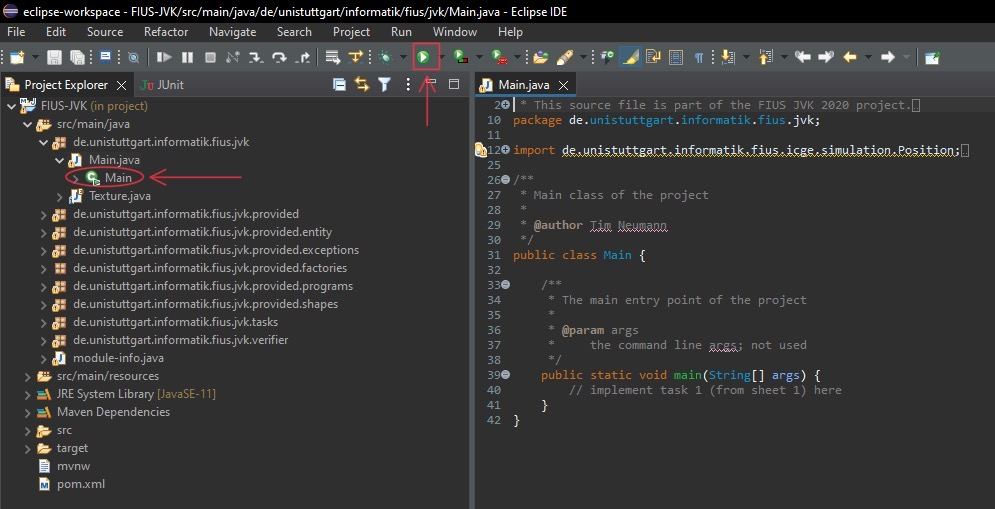
\includegraphics [width=1\textwidth]{./figures/ide.jpg}
			\caption{Erklärung zur Ausführung des Projekts}
		\end{figure}
    \end{itemize}
    \item Finde in der \lstinline{Main}-Klasse die Zeile mit\\
	\hspace*{\fill}\lstinline{// implement task 1 (from sheet 1) here}\hspace*{\fill}\\ und füge an seiner Stelle den fehlenden Code aus dem Bild unten ein.
    Aktuell musst du den Code noch nicht verstehen, es geht darum den Code Editor in Eclipse kennenzulernen.\\
    Achte auch darauf was passiert während du die fehlenden Zeilen eingibst.

	\begin{figure} [H]
		\centering
		\label{code}
		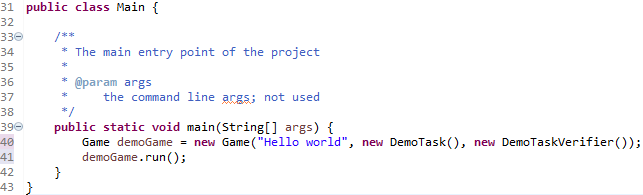
\includegraphics [width=0.66\textwidth]{./figures/code.1.png}
		\caption{Der einzufügende Code}
	\end{figure}

    Führe das Programm nun aus. Nun sollte ein Fenster mit der Simulator Ansicht auf dem Bildschirm auftauchen. Schau ihn Dir genau an, denn er wird dich wahrscheinlich die nächsten Tage begleiten.\\
    Suche als nächstes die (rote) Stop Taste \colorbox{red}{$\square$} in Eclipse um das Programm abzubrechen. Die Taste befindet sich in Eclipse unten in der Titelleiste der Console.
    \item Versuche nun den Code so zu verändern, dass dein Name im Fenstertitel steht.
\end{enumerate}


\begin{Infobox}[HowTo: Auskommentieren]
    Manchmal möchte man, dass ein bestimmter Code-Teil nicht ausgeführt wird.
    Vielleicht möchten man ihn erst später ausführen oder ihn einfach nicht verlieren.
    In solchen Fällen Kommentieren man die Code-Zeilen einfach aus.
    Dies geht, indem du in der Code-Zeile zwei Schrägstriche (\emph{eng.} slashes) (\lstinline{//}) voranstellst.\\
    Als Beispiel schaue dir folgenden Code an:\\

    \hfill
    \begin{minipage}{0.96\textwidth}
        \begin{lstlisting}
    public void run(Simulation sim) {
        PlayfieldModifier \ pm =
                new PlayfieldModifier(sim.getPlayfield());
        pm.placeEntityAt(new Coin(), new Position(0,0));
    }
        \end{lstlisting}
    \end{minipage}

    Wenn nun die letzte Zeile auskommentieren werden soll, in der ein \lstinline{Coin} Objekt an der Position \lstinline{0,0} auf dem Spielfeld platziert werden soll, dann verändert man den oberen Code wie folgt:\\

    \hfill
    \begin{minipage}{.96\textwidth}
        \begin{lstlisting}
    public void run(Simulation sim) {
        PlayfieldModifier pm =
                new PlayfieldModifier(sim.getPlayfield());
        //pm.placeEntityAt(new Coin(), new Position(0, 0));
    }
        \end{lstlisting}
    \end{minipage}

    Alles ab den zwei Schrägstrichen bis zum Zeilen Ende wird nun vom Computer ignoriert und damit nicht ausgeführt, was auch durch eine andere Färbung in Eclipse deutlich wird.
\end{Infobox}


\begin{Infobox}[Fehler]
    Einige Aufgaben in Blatt 1 (und auch auf den anderen Blättern) verlangen von dir den Code absichtlich kaputtzumachen.
    Das Ziel davon ist es das du die verschiedenen Fehler bereits kennenlernst.\\
    Achte also bei solchen Aufgaben darauf, welche Änderung zu welchem Fehler geführt hat.
    Falls du nun später einen Fehler beim Programmieren machst, kann dir dieses Wissen helfen den Code zu reparieren.\\
    Du brauchst auch keine Angst haben, dass du das importierte Projekt kaputt machen könntest.
    Eclipse hat eine \q{Undo}-Funktion welche Änderungen rückgängig macht.
    Diese findest du im Context-Menü oben unter \fbox{Edit}/\fbox{Bearbeiten} oder über das drücken von \fbox{Strg + Z}.\\
    Falls du trotzdem Hilfe brauchst, kannst (\emph{und sollst}) du dich gerne bei den Tutoren melden oder deinen Nachbarn/ deiner Nachbarin fragen.
\end{Infobox}


\begin{enumerate} \setcounter{enumi}{3}
\item Finde heraus was passiert, wenn man die erste oder die zweite Zeile in der Main-Funktion auskommentiert.\\
Hinweis: Nicht alle Varianten funktionieren zwangsläufig, Überlege warum dies der Fall sein könnte.
\item Vielleicht sind dir beim Ausprobieren in a) schon einige Dinge aufgefallen, die der Eclipse Editor anders macht als Textverarbeitungsprogramme, wie zum Beispiel Word.\\
Wenn du zum Beispiel \lstinline{demoGame.} eingibst, erscheint ein \textit{Overlay} mit möglichen \textit{Autocompletions}. Um in der erscheinenden Dokumentation (mit Beispielen) scrollen zu können, musst du einmal kurz \fbox{F2} drücken.\\
Wenn du dann mit der Maus über andere Stellen im Code hoverst, verschwindet das Overlay wieder.
Du kannst das \textit{Autocompletions}-Overlay öffnen manuell, indem du den Cursor direkt nach \lstinline{demoGame.} platzierst und \fbox{Strg + Space} (Space ist die Leertaste) drückst.
\item
Wenn du die Maus über \lstinline{Game} bewegst, siehst du ein Overlay mit der Dokumentation.
Das funktioniert auch an anderen Stellen im Code.
Was steht im Overlay von \lstinline{DemoTask()}? Sollte sich das Overlay nicht öffnen, dann kannst du auch \fbox{F2} drücken
\item
Wenn du \fbox{Strg + Shift + F} (Shift ist die Taste mit der man Großbuchstaben schreibt) drückst, formatiert Eclipse den Code für dich. Diese Funktion ist sehr nützlich, um den Überblick über deinen Code zu behalten und ihn besser lesbar zu machen.\\
Füge an verschiedenen Stellen neue Zeilen und Leerzeichen und zeilenumbrüche ein und beobachte was passiert, wenn du \fbox{Strg + Shift + F} drückst.
\end{enumerate}


\begin{Infobox}[Optionale Aufgaben]
    Aufgaben die mit \optional markiert, sind müssen nicht bearbeitet werden.
    Sie setzen schon Vorkenntnisse in Java oder Programmieren voraus und sind deshalb auch oft deutlich schwerer als die normalen Aufgaben.
    Wenn du also an einer optionalen Aufgabe festhängst, dann solltest du mit der nächsten normalen Aufgabe weitermachen.
    Später, wenn du genug Zeit oder Wissen hast um die optionale Aufgabe zu lösen, kannst du nochmal zu ihr zurückkehren.
\end{Infobox}


\begin{enumerate} \setcounter{enumi}{5}
\item \optional Finde eine Möglichkeit, den Fenstertitel nach der \lstinline{demoGame.run();} Zeile zu ändern.
Dafür benötigst du den folgenden Code, den du allerdings noch etwas anpassen musst:\\
\hspace*{\fill}\lstinline{demoGame.getGameWindow().setWindowTitle();}\hspace*{\fill}\\
$\rightarrow$ \textbf{Tipp:} Du musst der \lstinline{setWindowTitle()}-Methode einen \enquote{\textit{String}} als Parameter übergeben. Wenn Du dir nicht sicher bist, wie das funktioniert, kannst Du Dir den Code aus Teilaufgabe \ref{code} anschauen.

\item \optional Benenne \lstinline{demoGame} in \lstinline{myDemoGame} um.
Wenn du nur die eine Stelle \enquote{\lstinline{Game demoGame}} anpasst, wirst du eine Fehlermeldung bekommen.
Mache deine Änderung nochmal rückgängig und platziere den Cursor in dem Wort \lstinline{demoGame}.\\
Mit der Tastenkombination \fbox{Shift + Alt + R} kommst du in den \q{Refactor}-Modus, in dem du alle Vorkommen des Namens gleichzeitig umbenennen kannst.
Das Gleiche geht auch über Rechtsklick > \fbox{Refactor} > \fbox{Rename}.\\
Mit \fbox{Strg + Shift + l} kannst du eine \textit{Liste alle Tastenkombinationen} ansehen.
\item \optional Versuche, drei Fenster gleichzeitig zu starten.
\end{enumerate}
